
\begin{center}
\Huge
Vækst af eksponentialfunktioner
\end{center}
\section*{Vækstrate og fremskrivningsfaktor}
\stepcounter{section}

Vi starter med en definition af en eksponentialfunktion
\begin{defn}[Eksponentialfunktion]
	Lad $a,b>0$. Så definerer vi en funktion $f$ på formen 
	\begin{align*}
		f(x) = b\cdot a^x
	\end{align*}
	til at være en \textit{eksponentialfunktion} med \textit{begyndelsesværdi} $b$. 
\end{defn}

Det er ikke svært at se, hvorfor $b$ kaldes for begyndelsesværdien thi
\begin{align*}
	f(0) = b\cdot a^0 = b\cdot 1 = b.
\end{align*}

\begin{exa}\label{exa:exa1}
Lad os betragte delingen af en bakterie. Vi starter med 1 bakterie, der efter én time er 2 bakterier, efter 2 timer er 4 bakterier, efter 3 timer er 8 bakterier osv. Denne situation kan beskrives ved eksponentialfunktionen $L(x)$ givet ved
\begin{align*}
L(x) = 2^x.
\end{align*}
De første 10 funktionsværdier kan ses af Fig. \ref{fig:sildebenfold}
\begin{figure}[H]
\center
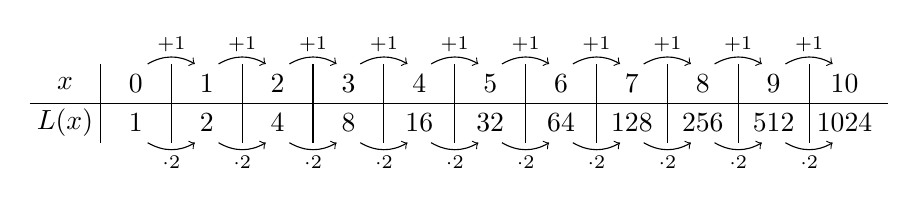
\begin{tikzpicture}
\foreach \i in {0,...,10}{
\draw (\i*0.9,0) -- (\i*0.9,1);
}
\draw (-0.9,0.5) -- (10,0.5);
\foreach \i in {0,...,10}{
\node at (\i*0.9+ 0.45,0.75) {$\i$};
\node at (\i*0.9+0.45,0.25) {$\fpeval{2^{\i}}$};
}
\node at (-0.45,0.75) {$x$};
\node at (-0.45,0.25) {$L(x)$};
\foreach \i in {0,...,9}{
\draw [->] (\i*0.9+0.6,1) to [out=30,in=150] (\i*0.9+1.2,1);
\node at (\i*0.9+0.9,1.25) {$\scriptstyle+1$};
\draw [->] (\i*0.9+0.6,-0) to [out=-30,in=-150] (\i*0.9+1.2,-0);
\node at (\i*0.9+0.9,-0.25) {$\scriptstyle\cdot 2$};
}
\end{tikzpicture}
\caption{De første ti funktionsværdier af $L$, der beskriver antallet af bakterier. }
\label{fig:sildebenfold}
\end{figure}
På Fig \ref{fig:flagxfold} kan grafen for $L$ ses. 
\begin{figure}[H]
\center
\begin{tikzpicture}
	\begin{axis}[axis lines=left,
		xlabel = {$x$ (Timer)},
		ylabel = {$y$ (Bakterier)}]
		\addplot[color=blue!40,thick, domain=0:10,samples=1000]{2^x};
	\end{axis}
\end{tikzpicture}
\caption{Antal bakterier som funktion af tiden}
\label{fig:flagxfold}
\end{figure}
\end{exa}
Inspriret af Eksempel \ref{exa:exa1} vil vi se på, hvordan eksponentiel vækst udvikler sig. Vi husker på, at en eksponentialfunktion $f$ kan skrives på formen
\begin{align*}
f(x) = b\cdot a^x.
\end{align*}
Ser vi på Fig. \ref{fig:sildebenfold}, så kan vi se, at vi i det tilfælde øger $f(x)$ med en faktor $2$, når vi øger $x$ med 1. Tilsvarende vil vi øge generel eksponentiel vækst med en faktor $a$, når vi øger $x$ med 1. Faktoren $a$ kaldes for fremskrivningsfaktoren. Vi kan se dette fænomen af Fig. \ref{fig:sildegen}
\begin{figure}[H]
\center
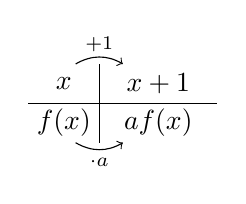
\begin{tikzpicture}
\foreach \i in {0}{
\draw (\i*0.9,0) -- (\i*0.9,1);
}
\draw (-0.9,0.5) -- (1.5,0.5);
\foreach \i in {0}{
\node at (\i*0.9+ 0.75,0.75) {$x+1$};
\node at (\i*0.9+0.75,0.25) {$af(x)$};
}
\node at (-0.45,0.75) {$x$};
\node at (-0.45,0.25) {$f(x)$};
\foreach \i in {0}{
\draw [->] (\i*0.9-0.3,1) to [out=30,in=150] (\i*0.9+0.3,1);
\node at (\i*0.9,1.25) {$\scriptstyle+1$};
\draw [->] (\i*0.9-0.3,-0) to [out=-30,in=-150] (\i*0.9+0.3,-0);
\node at (\i*0.9,-0.25) {$\scriptstyle\cdot a$};
}
\end{tikzpicture}
\caption{Udvikling af eksponentiel vækst.}
\label{fig:sildegen}
\end{figure}
Det er ikke svært at vise, at dette rent faktisk er sandt. Betragter vi
\begin{align*}
f(x+1) = ba^{x+1} = ba^xa = af(x),
\end{align*}
så ses det, at eksponentialfunktioner har en sådan udvikling. 
\begin{defn}[Vækstrate og fremskrivningsfaktor]
	For en eksponentialfunktion $f$ givet ved
	\begin{align*}
		f(x) = b\cdot a^x
	\end{align*}
	kaldes $a$ for \textit{fremskrivningsfaktoren.}
	Vi definerer desuden \textit{vækstraten} $r$ som
	\begin{align*}
		r = a -1.
	\end{align*}
\end{defn}

\section*{Opgave 1}

\begin{enumerate}[label=\roman*)]
	\item En eksponentialfunktion $f$ er givet ved
	\begin{align*}
		f(x) = 1.3\cdot 0.97^x.
	\end{align*}
	Bestem fremskrivningsfaktoren og vækstraten for $f$. Afgør desuden hvor mange procent $f$ stiger/falder med, hvis $x$ øges med 1.
	\item En eksponentialfunktion $f$ er givet ved
	\begin{align*}
		f(x) = b\cdot 2^x.
	\end{align*}
	Bestem fremskrivningsfaktoren og vækstraten for $f$. Afgør desuden hvor mange procent $f$ stiger/falder med, hvis $x$ øges med 1.
	\item En eksponentialfunktion $f$ er givet ved
	\begin{align*}
		f(x) = 9\cdot 1.34^x.
	\end{align*}
	Bestem fremskrivningsfaktoren og vækstraten for $f$. Afgør desuden hvor mange procent $f$ stiger/falder med, hvis $x$ øges med 1.
	\item En eksponentialfunktion $f$ er givet ved
	\begin{align*}
		f(x) = \sqrt{2}\cdot 5^x.
	\end{align*}
	Bestem fremskrivningsfaktoren og vækstraten for $f$. Afgør desuden hvor mange procent $f$ stiger/falder med, hvis $x$ øges med 1.
\end{enumerate}

\section*{Opgave 2}
\begin{enumerate}[label=\roman*)]
	\item Udfyld følgende tabel og opskriv derefter forskriften for eksponentialfunktionen $f$.
	\item Undersøg, om du har udfyldt tabellen korrekt ved at bestemme $f(10)$. 
\end{enumerate}

\begin{center}
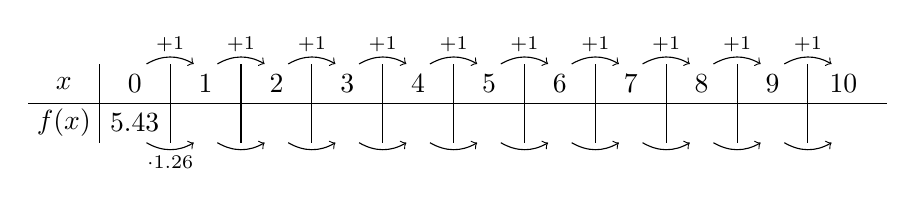
\begin{tikzpicture}
\foreach \i in {0,...,10}{
\draw (\i*0.9,0) -- (\i*0.9,1);
}
\draw (-0.9,0.5) -- (10,0.5);
\foreach \i in {0,...,10}{
\node at (\i*0.9+ 0.45,0.75) {$\i$};
}
\node at (0.45,0.25) {$5.43$};
\node at (-0.45,0.75) {$x$};
\node at (-0.45,0.25) {$f(x)$};
\foreach \i in {0,...,9}{
\draw [->] (\i*0.9+0.6,1) to [out=30,in=150] (\i*0.9+1.2,1);
\node at (\i*0.9+0.9,1.25) {$\scriptstyle+1$};
\draw [->] (\i*0.9+0.6,-0) to [out=-30,in=-150] (\i*0.9+1.2,-0);
}
\node at (0.9,-0.25) {$\scriptstyle\cdot 1.26$};
\end{tikzpicture}
\end{center}

\section*{Opgave 3}

\begin{enumerate}[label=\roman*)]
	\item Lad $f$ være givet ved
	\begin{align*}
		f(x) = 5\cdot 1.7^x.
	\end{align*}
	Hvor mange procent øges $f$ med, hvis $x$ øges med 2?
	\item Lad $f$ være givet ved
	\begin{align*}
		f(x) = b\cdot 0.77^x.
	\end{align*}
	Det oplyses, at $f(4) = 6.01$. Bestem $f(8)$. 
	\item Lad $f$ være givet ved
	\begin{align*}
		f(x) = 9.99 \cdot 1.05^x.
	\end{align*}
	Hvor meget skal $x$ øges med før $f$ fordobles?
\end{enumerate}


\section*{Opgave 4}
\begin{enumerate}[label=\roman*)]
	\item Hvis vi folder et stykke papir $25$ gange, hvor mange lag papir har vi så?
 	\item Hvis ét lag papir er 0.1mm tykt, hvor tykt er dette stykke foldede papir?
	\item Hvor mange gange skal vi folde papiret, for at det bliver 1km tykt?
\end{enumerate}
\section*{Opgave 5}
\begin{enumerate}[label=\roman*)]
\item En bakteriekoloni indeholder til tid $t=0$ $B_0 = 100.000$ bakterier. En bakterie deler sig i gennemsnit 1 gang per 4. time, og bakteriekolonien har ubegrænset plads. Beskriv antallet af bakterier som funktion af tiden i timer. Hvor mange bakterier er der i kolonien efter et døgn? Hvornår er der 1 mia. $(10^9)$ bakterier i kolonien?
\item Et glas vand stilles i et rum, og temperaturen i vandet antages at kunne beskrives ved
\begin{align*}
H(t) = 70\cdot(0.97)^t,
\end{align*}
hvor $H(t)$ beskriver temperaturen i grader celcius og $t$ betegner tiden i minutter. Hvor varmt er vandet, når det stilles ind i rummet? Hvor varmt er det efter 5 minutter? Hvor varmt er der i rummet i følge modellen. 
\end{enumerate}

\section*{Opgave 6}
\begin{enumerate}[label=\roman*)]
\item Bevis, at hvis vi øger $x$ med 2 i en eksponentialfunktion $f(x)$, så tilsvarer dette at øge $f(x)$ med en faktor $a^2$. Hvad hvis vi øger $x$ med $3$?
\item Bevis, at hvis vi øger $x$ med $n$ i en eksponentialfunktion $f(x)$, så tilsvarer dette at øge $f(x)$ med en faktor $a^n$.
\end{enumerate}